\section{Preliminary Work}
In this section, we present our concurrent garbage collection algorithm.
%The pseudocode description of our collector is given in Algorithms \ref{algorithm:linkset}--\ref{algorithm:cleanup}.
Each object in the heap contains three reference counts: the first
two are the strong and weak, the third is the phantom count. Each object also
contains a bit named {\tt which} (Brownbridge \cite{Brownbridge1985} called it the ``strength-bit'')
to identify which of the first two counters is
used to keep track of strong references, as well as a boolean called {\tt
phantomized} to keep track of whether the node is phantomized.
Outgoing links (i.e., pointers) to other objects must also contain (1) a {\tt which} bit to
identify which reference counter on the target object they increment, and (2) a {\tt
phantom} boolean to identify whether they have been phantomized. This data structure for each object can be seen in the example given in Fig.~\ref{ex1}.

Local creation of links only allows the creation of strong references when no
cycle creation is possible. Consider the creation of a link from a source object $S$
to a target object $T$. The link will be created strong if (i) the only strong
links to $S$ are from roots i.e. there is no object $C$ with a strong link to $S$;
(ii) object $T$ has no outgoing links i.e. it is newly created and its outgoing links are
not initialized; and (iii) object $T$ is phantomized, and $S$ is not. All
self-references are weak. Any other link is created phantom or weak.
%See Algorithm~\ref{algorithm:linkset}.

To create a strong link, the {\tt which} bit on the link must match the value of
the {\tt which} bit on the target object. A weak link is created by setting the
{\tt which} bit on the reference to the complement of the value of the {\tt
which} bit on the target.

When the strong reference count on any object reaches zero, the garbage
collection process begins.
If the object's weak reference count is zero, the
object is immediately reclaimed. If the weak count is positive, then a
a sequence of three phases is initiated: $Phantomization$, $Recovery$, and $CleanUp$.
In $Phantomization$, the object toggles its {\tt which} bit, turning its
incoming weak reference counts to strong ones,
and phantomizes its outgoing links.
%See Algorithm~\ref{algorithm:linkfree}.

Phantomizing a link transfers a reference count (either strong or weak), to the
phantom count on the target object. If this causes the object to lose its
last strong reference, then the object may also phantomize, i.e. toggle its {\tt which} bit (if that
will cause it to gain strong references), %see Algorithm~\ref{algorithm:phantomizenode}),
and phantomizes all its outgoing
links. This process may spread to a large number of target objects.
%See Algorithm~\ref{algorithm:phantomizelink}.

All objects touched in the process of a phantomization that were able to recover
their strong references by toggling their {\tt which} bit are remembered and put
in a ``recovery list''.
%(see Algorithm~\ref{algorithm:main}).
When phantomization is finished, $Recovery$ begins, starting with all objects in the recovery list.

To perform a recovery, the system looks at each object in the recovery list,
checking to see whether it still has a positive strong reference count. If it
does, it sets the {\tt phantomized} boolean to false, and rebuilds its outgoing
links, turning phantoms to strong or weak according to the rules above. If a
phantom link is rebuilt and the target object regains its first strong reference
as a result, the target object sets its {\tt phantomized} boolean to false and
attempts to recover its outgoing phantom links (if any). The recovery continues
to rebuild outgoing links until it terminates. %See Algorithm~\ref{algorithm:rebuild}.

Finally, after the recovery is complete, $CleanUp$ begins. The recovery list is revisited a second
time. Any objects that still have no strong references are deleted. %See Algorithm~\ref{algorithm:cleanup}.

Note that all three of these phases, $Phantomization$, $Recovery$, and $CleanUp$ are,
by their definitions, linear in the number of links; we prove this formally in Theorem \ref{theorem:termination} in Section \ref{section:correctness}. Links can undergo only one
state change in each of these phases: strong or weak to phantom during
$Phantomization$, phantom to strong or weak during $Recovery$, and phantom to
deleted in $CleanUp$. 

We now present some examples to show how our algorithm performs collection in several real word scenarios.


\subsection{Example: A Simple Cycle}

In Fig.~\ref{ex1} we see a cyclic graph with three nodes. This figure shows
the counters, bits, and boolean values in full detail to make it clear how
these values are used within the algorithm. Objects are represented with
circles, links have a pentagon with state information at their start and
an arrow at their end.

In Step 0, the cycle is supported by a root, a reference from stack or global
space. In Step 1, the root reference is removed, decrementing the strong
reference by one, and beginning a $Phantomization$. Object C toggles its which pointer and
phantomizes its outgoing links. Note that toggling the which pointer causes the
link from A to C to become strong, but nothing needs to change on A
to make this happen.

In Step 2, object B also toggles its which bit, and phantomizes its
outgoing links. Likewise, in Step 3, object A phantomizes, and the
$Phantomization$ phase completes.

$Recovery$ will attempt to unphantomize objects A, B, and C. None of them,
however, have any strong support, and so none of them recover.

$Cleanup$ happens next, and all objects are reclaimed.


\begin{figure*}[!t]
  \centering
  {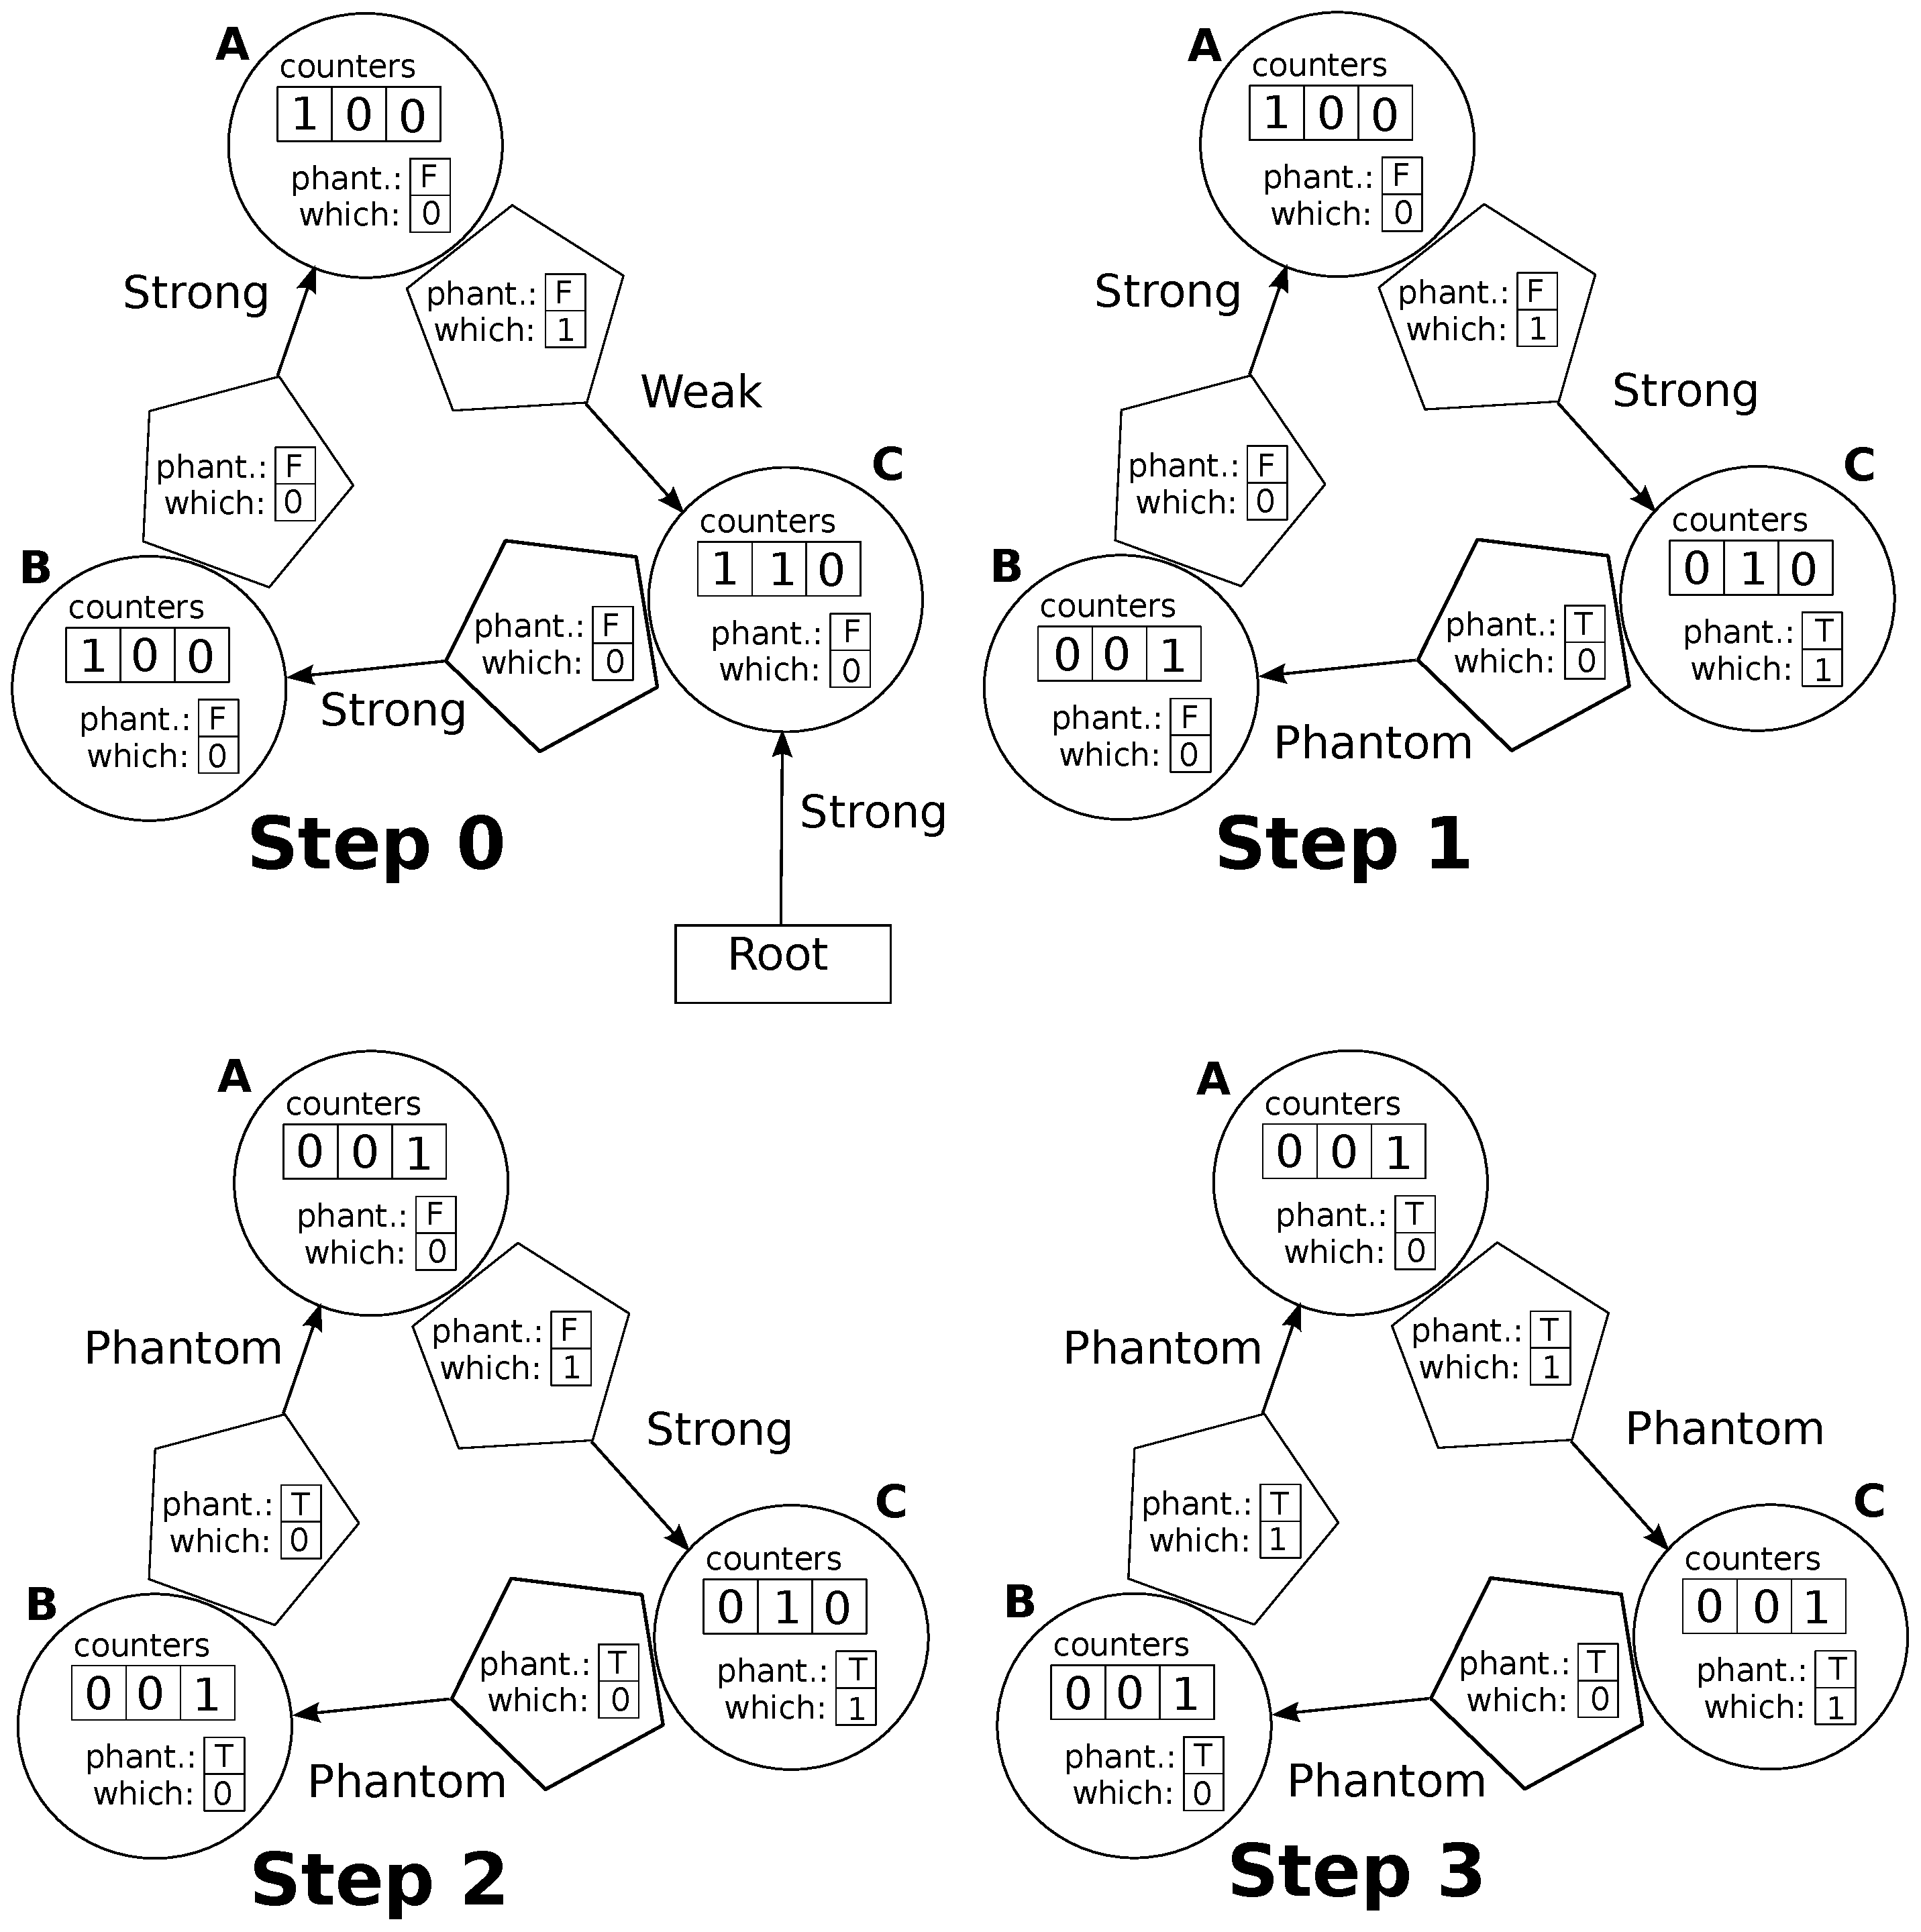
\includegraphics[height=4.5in]{figs/method}\label{fig:example1}}
  \caption{Reclaiming a cycle with three objects}%
  \label{ex1}
\end{figure*}

\begin{figure*}[!t]
  \centering
  {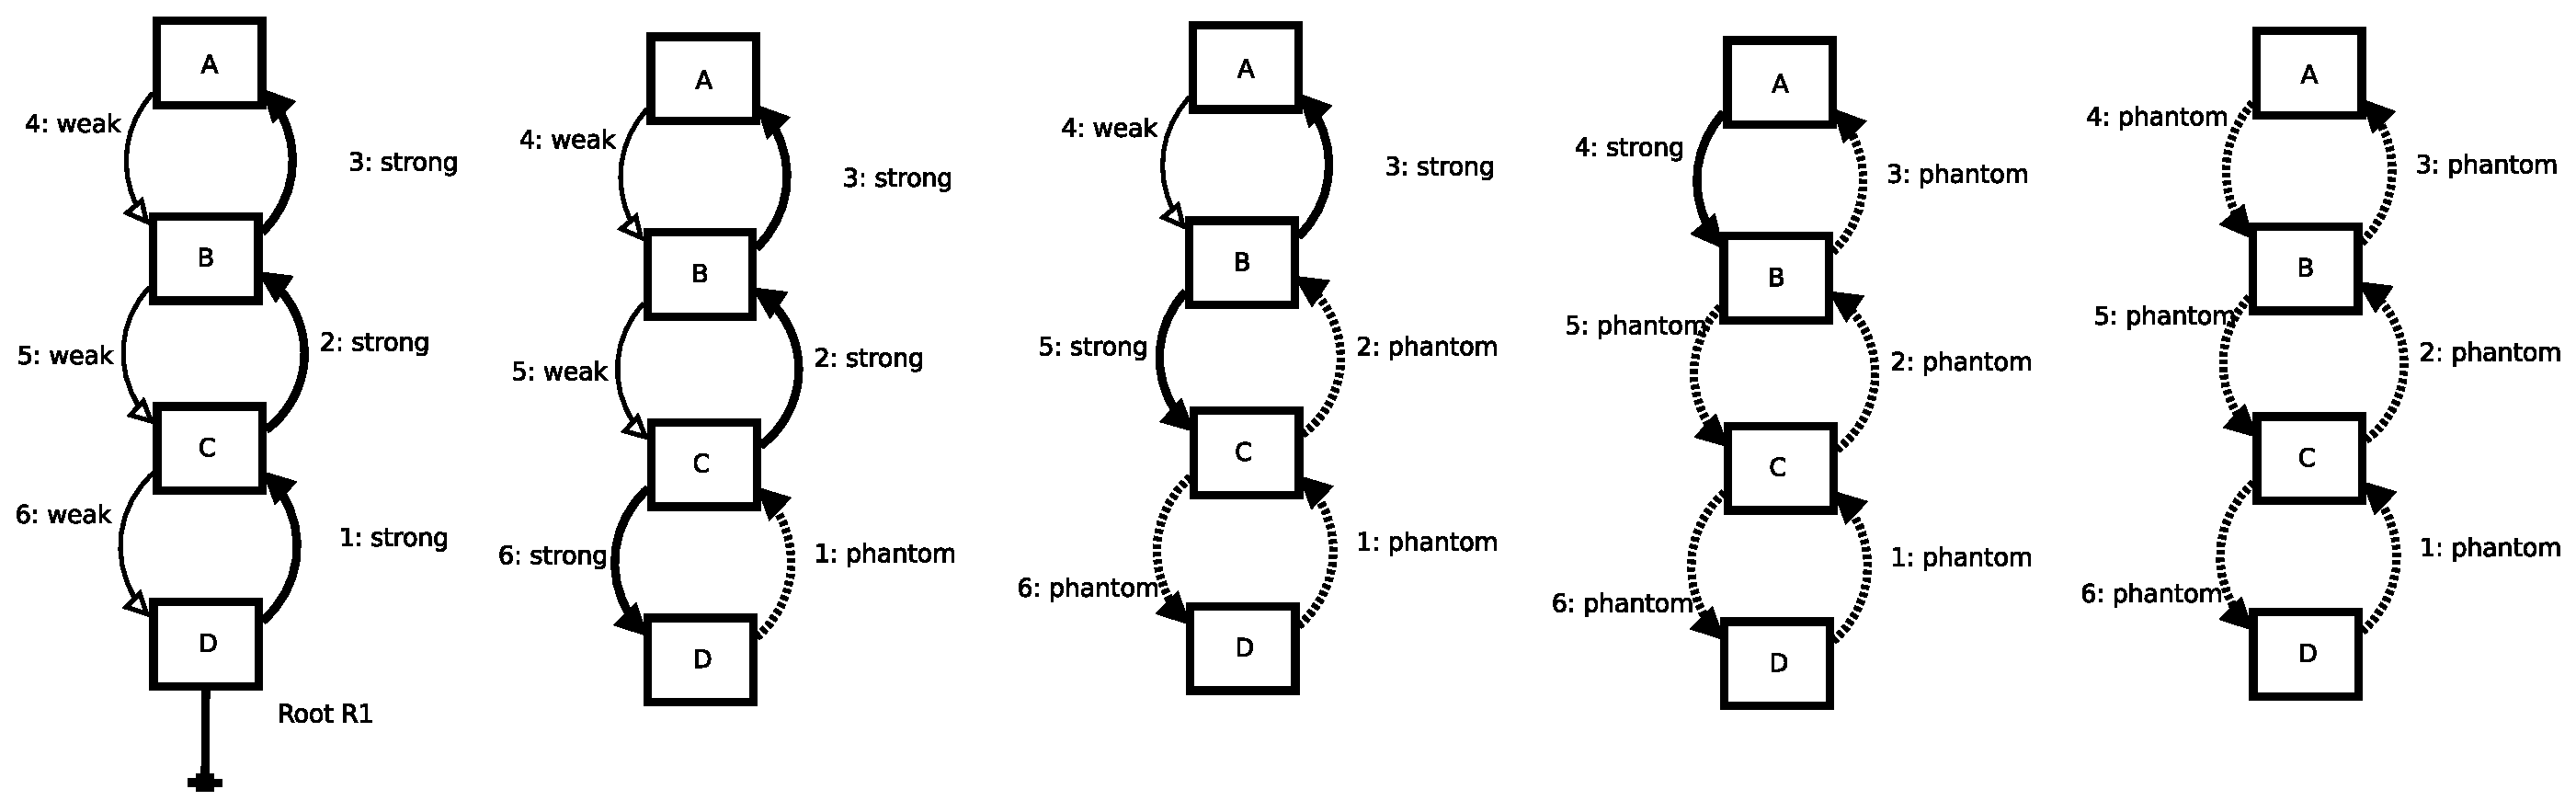
\includegraphics[height=2.0in]{figs/doublylinkedlist}\label{fig:example2}}
 \caption{Doubly-linked list}%
  \label{ex2}
\end{figure*}




\begin{figure*}[!t]
  \centering
  {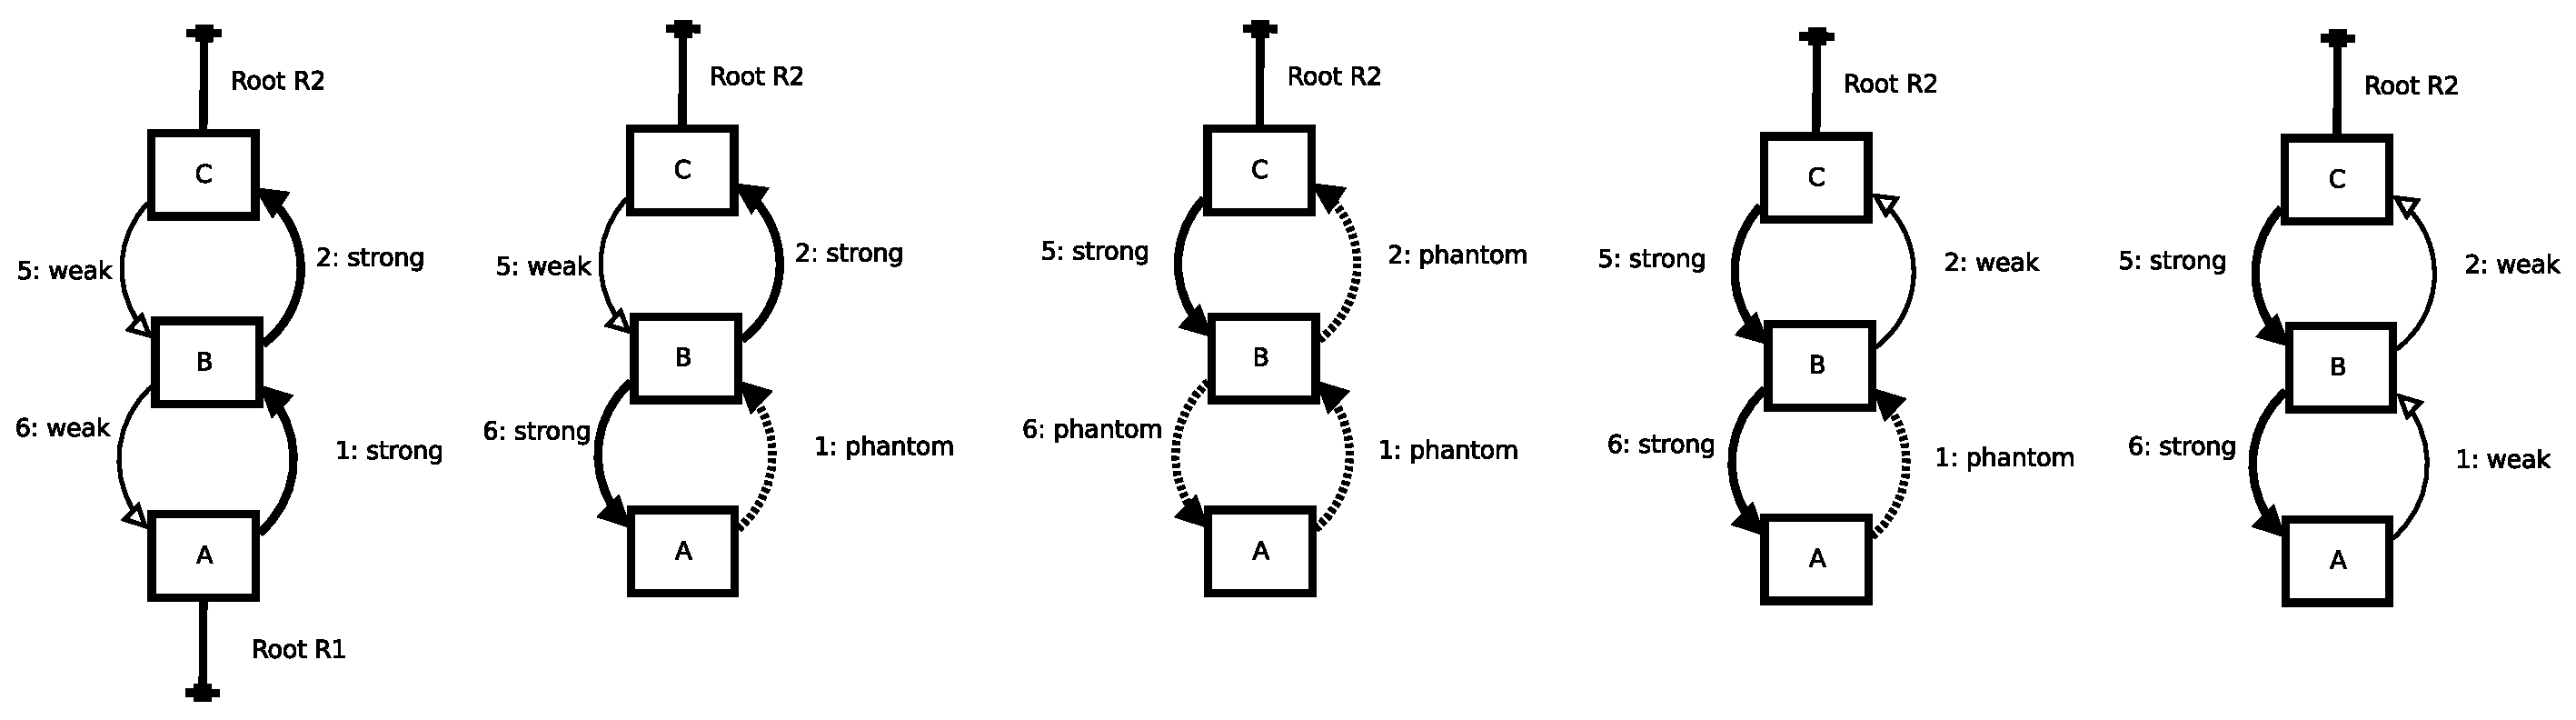
\includegraphics[height=2.0in]{figs/recoveringdbl}}%\label{fig:example1}}
  \caption{Rebalancing a doubly-linked list}%
  \label{ex3}
\end{figure*}


\subsection{Example: A Doubly-Linked List}

The doubly linked list depicted in Fig.~\ref{ex2} is a classic
example for garbage collection systems. The structure consists of
6 links, and the collector marks all the links as phantoms in 8
steps.

This figure contains much less detail than Fig.~\ref{ex1}, which
is necessary for a more complex figure.




\subsection{Example: Rebalancing A Doubly-Linked List}

Fig.~\ref{ex3} represents a worst case scenario for our algorithm. As a
result of losing root $R1$, the
strong links are pointing in exactly the wrong direction to provide
support across
an entire chain of double links. During $Phantomization$, each
of the objects in the list must convert its links to phantoms,
but nothing is deleted. $Phantomization$ is complete in the third
figure from the left, and $Recovery$ begins.
The fourth step in the figure, when link 6 is converted from phantom to weak
marks the first phase of the recovery.



\subsection{Example: Recovering Without Detecting a Cycle}

In Fig.~\ref{prove} we see the situation where the collector recovers from the
loss of a strong link without searching the entire cycle. When root $R1$ is removed,
node $A$ becomes phantomized. It turns its incoming link (link $1$) to strong,
and phantomizes its outgoing link (link $2$), but
then the phantomization process ends. Recovery is successful, because $A$ has strong
support, and it rebuilds its outgoing link as weak. At this point, collection
operations are finished.

Unlike the doubly-linked list example above, this case describes an optimal
situation for our garbage collection system.

\subsection{Concurrency Issues}

%Note that the algorithm section omits the actual calls to lock and unlock present in our fine-grained parallel prototype.
This section provides details of the implementation.
%A reference implementation is also provided ~\cite{url:refimpl}.\todo{Make public repo}
%\update{What about we provide implementation link here. Currently it is withheld for supporting double-blind review. I think the link will make our case stronger and it does not reveal our identity directly.}

\subsection{The Single-Threaded Collector}
There are several methods by which the collector may be
allowed to interact concurrently with a live system. The first, and most straightforward
implementation, is to use a single garbage collection thread to manage nontrivial
collection operations. This technique has the advantage of limiting the amount
of computational power the garbage collector may use to perform its work.

For the collection process to work, phantomization must run to completion before
recovery is attempted, and recovery must run to completion before cleanup can
occur. To preserve this ordering in a live system,
whenever an operation would remove the last strong link
to an object with weak or phantom references, the link is instead transferred
to the collector, enabling it to perform phantomization at an appropriate time.
%See Algorithms.~\ref{algorithm:linkfree} and~\ref{algorithm:addtocollector}.

%In Algorithm~\ref{algorithm:addtocollector}, we see that
After the strong link is processed, the garbage collector needs to create a phantom
link to hold onto the object while it performs its processing, to ensure the
collector itself doesn't try to use a deleted object.

Another point of synchronization is the creation of new links. If the
source of the link is a phantomized node, the link is created in the phantomized
state. %See Algorithm~\ref{algorithm:linkset}.

With these relatively straightforward changes, the single-threaded garbage collector
may interact freely with a live system.

%Note that in the following sections, locks are always obtained in canonical order that avoids deadlocks. Unlock methods unlock the last set of items that were locked.

The lists on the collectors are thread-safe.

The collector object is itself managed by a simple reference count. Code for incrementing and decrementing this count is not explicitly present in the code below.

A reference implementation is also provided ~\cite{url:refimpl}.

\begin{algorithm}[H]
		\scriptsize
			\caption{LinkSet creates a new link,
				and decides the type of the link to create.}
			\label{single:algorithm:linkset}
			
%				\begin{multicols}{2}
					\begin{algorithmic}[1]
		
%{\small
%\tcp{}
\Procedure{ LinkSet(link,node)}{}
\State lock (link.Source,node)
\If {node $==$ NULL}
\State LinkFree(link)
\State link.Target = NULL
\EndIf
\If {link.Target $==$ node }
\State Return
\EndIf
\State oldLink = copy(link) 
\State link.Target = node
\If {link.Source.Phantomized }
\State MergeCollectors(link.Source, link.Target)
\State link.PhantomCount++
\State link.Phantomized = True
\ElsIf {link.Source == node }
\State link.Which = 1 - node.Which
\State node.Count[link.Which]++
\ElsIf { node.Links not initialized }
\State node.Count[link.Which]++
\State link.Which = node.Which
\Else
\State link.which = 1 - node.Which
\State node.Count[link.Which]++
\EndIf
\If { oldLink != NULL}
\State LinkFree(oldLink)
\EndIf
\State unlock()
\EndProcedure
%}
%\caption{LinkSet}
%\label{}
\end{algorithmic}
%\end{multicols}
\end{algorithm}
\setlength{\textfloatsep}{0pt}

\begin{algorithm}[H]
	\scriptsize

%	\begin{multicols}{2}
		\begin{algorithmic}[1]

\Procedure{ LinkFree(link)}{}

% \tcp*[f]{Create a pointer from object $R$ to some free object}

\State lock(link.Source,link.Target)
\If { link.Target == NULL }
\State Return
\EndIf
\If { link.Phantomized }
\State DecPhantom(link.Target)
\Else
\State link.Target.Count[link.Which]-\,-
\If { link.Target.Count[link.Which] == 0 {\bf And} 
 link.Target.Which == link.Which }
\If { link.Target.Count[1-link.Target.Which] == 0 {\bf And} 
 link.Target.PhantomCount == 0 }
\State Delete(node)
\State link.Target = NULL
\Else
\If { link.Target.Collector == NULL }
\State link.Target.Collector = new Collector()
\EndIf
\State AddToCollector(link.Target)
\EndIf
\EndIf
\EndIf
\State unlock()

\EndProcedure

\caption{LinkFree}
\label{algorithm:linkfree}
\end{algorithmic}
%\end{multicols}
\end{algorithm}


\setlength{\textfloatsep}{0pt}
\begin{algorithm}[H]
		\scriptsize
		
%		\begin{multicols}{2}
			\begin{algorithmic}[1]
				
%{\small
%\begin{multicols}{2}
% \tcp{$R$ and $S$ are objects currently in use.}
% \tcp*[f]{Create a pointer from object $R$ to some free object}


%\tcp{Adding an object to the collector puts back the strong
%count, effectively transferring the source of the strong link
%to the collector. It also adds a phantom count, which helps
%prevent the clearing of the Collector field.}

\Procedure {AddToCollector(node)}{}
%{\Indp
\While { True }
\State lock(node,node.Collector)
\If {node.Collector.Forward != NULL }
\State node.Collector = node.Collector.Forward
\Else
\State node.Count[node.Which]++
\State node.PhantomCount++
\State node.Collector.CollectionList.append(node)
\State Break
\EndIf
\State{unlock()}
\EndWhile
%}
\EndProcedure
%}
\caption{AddToCollector}
\label{single:algorithm:addtocollector}
\end{algorithmic}
%\end{multicols}
\end{algorithm}
%\end{multicols}


\setlength{\textfloatsep}{0pt}
\begin{algorithm}[H]
	\scriptsize
	
%	\begin{multicols}{2}
		\begin{algorithmic}[1]
%{\small
%\begin{multicols}{2}
%\tcp{The collector takes away the strong link it made in
%AddToCollector().}
\Procedure { PhantomizeNode(node,collector)}{}
%{\Indp
\State {lock(node)}
\While { collector.Forward != NULL }
\State collector = collector.Forward
\EndWhile
\State node.Collector = collector
\State node.Count[node.Which]-\,-
%\State// Prevent deletion while the
%\State// node is managed by the Collector
\State phantomize = False
\If { node.Count[node.Which] $>$ 0 }
\State {\bf Return}
\Else
\If { node.Count[1-node.Which] $>$ 0 }
\State node.Which = 1-node.Which
\EndIf
\If { {\bf Not} node.Phantomized }
\State node.Phantomized = True
\State node.PhantomizationComplete = False
\State phantomize = True
\EndIf
\EndIf
\State links = NULL 
\If { phantomize }
\State links = copy(node.Links)
\EndIf
\State {unlock()}
\For { each outgoing link in links }
\State PhantomizeLink(link)
\EndFor
\State lock(node)
\State {node.PhantomizationComplete = True}
\State unlock()
%}
\EndProcedure
%\end{multicols}
%}
\caption{PhantomizeNode}
\label{algorithm:phantomizenode}
\end{algorithmic}
%\end{multicols}
\end{algorithm}



\setlength{\textfloatsep}{0pt}
\begin{algorithm}[H]
	\scriptsize
	
%	\begin{multicols}{2}
		\begin{algorithmic}[1]
%{\small
%\begin{multicols}{2}
%\tcp{This method describes the
%work to be carried out by a
%garbage collection thread. Live
%objects pointing to this collector, or
%Forward pointers from other collectors
%contribute to the RefCount field on
%the Collector.}
\Procedure { Collector.Main()}{}
%{\Indp
\While { True }
\State WaitFor(Collector.RefCount == 0 {\bf Or} Work to do)
\If { Collector.RefCount == 0 {\bf And} No work to do }
\State {\bf Break}
\EndIf
\While { Collector.MergedList.size() $>$ 0 }
\State node = Collector.MergedList.pop()
\State Collector.RecoveryList.append(node)
\EndWhile
\While { Collector.CollectionList.size() $>$ 0 }
\State node = Collector.CollectionList.pop()
\State PhantomizeNode(node,Collector)
\State Collector.RecoveryList.append(node)
\EndWhile
\While { Collector.RecoveryList.size() $>$ 0 }
\State node = Collector.RecoveryList.pop()
\State RecoverNode(node)
\State Collector.CleanList.append(node)
\EndWhile
\While {Collector.RebuildList.size() $>$ 0 }
\State node = Collector.RebuildList.pop()
\State RecoverNode(node)
\EndWhile
\While {Collector.CleanList.size() $>$ 0 }
\State node = Collector.CleanList.pop()
\State CleanNode(node)
\EndWhile
\EndWhile
%}
\EndProcedure
%}
\caption{Collector.Main}
\label{algorithm:main}
\end{algorithmic}
%\end{multicols}
\end{algorithm}
\setlength{\textfloatsep}{0pt}


\begin{algorithm}[H]
	\scriptsize
	
%	\begin{multicols}{2}
		\begin{algorithmic}[1]
%{\small
%\begin{multicols}{2}
\Procedure {PhantomizeLink(link)}{}
%{\Indp
\State {lock(link.Source,link.Target)}
\If { link.Target == NULL }
\State {unlock()}
\State {\bf Return}
\EndIf
\If { link.Phantomized }
\State {unlock()}
\State{\bf Return} 
\EndIf
\State link.Target.PhantomCount++
\State link.Phantomized = True
\State linkFree(link)
\State MergeCollectors(link.Source, link.Target)
\State  {unlock()}
%}
\EndProcedure
%}
\caption{PhantomizeLink}
\label{single:algorithm:phantomizelink}
\end{algorithmic}
%\end{multicols}
\end{algorithm}



\setlength{\textfloatsep}{0pt}
\begin{algorithm}[H]
	\scriptsize
	
%	\begin{multicols}{2}
		\begin{algorithmic}[1]
%{\small
%\begin{multicols}{2}
%\tcp{DecPhantom is responsible for removing any reference to
%the collector.}
\Procedure { DecPhantom(node)}{}
%{\Indp
\State  {lock(node)}
\State node.PhantomCount- -
\If { node.PhantomCount == 0 }
\If { node.Count[node.Which]== 0 {\bf And}
 node.Count[1-node.Which] == 0 }
\State Delete(node)
\Else
\State node.Collector = NULL
\EndIf
\EndIf
\State {unlock()}
%}
\EndProcedure
%}
\caption{DecPhantom}
\label{single:algorithm:decPhantom}
\end{algorithmic}
%\end{multicols}
\end{algorithm}
\setlength{\textfloatsep}{0pt}



\begin{algorithm}[H]
	\scriptsize
	
%	\begin{multicols}{2}
		\begin{algorithmic}[1]
%{\small
%\begin{multicols}{2}
\Procedure {RecoverNode(node)}{}
%{\Indp
\State  {lock(node)}
\State links = NULL
\If { node.Count[node.Which] $>$ 0 }
\State WaitFor(node.PhantomizationComplete == True)
\State node.Phantomized = False
\State links = copy(node.Links)
\EndIf
\State {unlock()}
\For {each  link in links }
\State Rebuild(link)
\EndFor
\EndProcedure
%}
%}
\caption{RecoverNode}
\label{algorithm:recover}
\end{algorithmic}
%\end{multicols}
\end{algorithm}
\setlength{\textfloatsep}{0pt}



\begin{algorithm}[H]
	\scriptsize
	
%	\begin{multicols}{2}
		\begin{algorithmic}[1]
%{\small
%\begin{multicols}{2}
\Procedure { Rebuild(link)}{}
%{\Indp
\State {lock(link.Source,link.Target)}
\If {link.Phantomized }
\If { link.Target == link.Source }
\State link.Which = 1- link.Target.Which
\ElsIf { link.Target.Phantomized } 
\State link.Which = link.Target.Which
\ElsIf { count(link.Target.Links) == 0 }
\State link.Which = link.Target.Which
\Else
\State link.Which = 1-link.Target.Which
\EndIf
\State link.Target.Count[link.Which]++
\State link.Target.PhantomCount- -
\If { link.Target.PhantomCount == 0 }
\State link.Target.Collector = NULL
\EndIf
\State link.Phantomized = False 
\State Add link.Target to Collector.RecoveryList
\EndIf
\State {unlock()}
 \EndProcedure
%}
%}
\caption{Rebuild}
\label{single:algorithm:rebuild}

\end{algorithmic}
%\end{multicols}
\end{algorithm}
\setlength{\textfloatsep}{0pt}


\begin{algorithm}[H]
	\scriptsize
	
%	\begin{multicols}{2}
		\begin{algorithmic}[1]
%{\small
%\begin{multicols}{2}
%\tcp{After deleting all the outgoing links, decrement
%the phantom count by one (i.e. the reference held by
%the collector itself). When the last phantom count
%is gone, the object is cleaned up.}
\Procedure {  CleanNode(node)}{}
%{\Indp
\State {lock(node)}
\State die = False
\If { node.Count[node.Which]== 0 {\bf And}
 node.Count[1-node.Which]== 0 }
\State die = True
\EndIf
\State {unlock()}
\If { die }
\For {each link in node }
\State LinkFree(link)
\EndFor
\EndIf
\State DecPhantom(node)
\EndProcedure
% }
%}
\caption{CleanNode}
\label{algorithm:cleanup}
\end{algorithmic}
%\end{multicols}
\end{algorithm}
\setlength{\textfloatsep}{0pt}


\begin{algorithm}[H]
	\scriptsize
	
%	\begin{multicols}{2}
		\begin{algorithmic}[1]
%{\small
\Procedure {  Delete(node)}{}
%{\Indp
\For {each link in node }
\State LinkFree(link)
\EndFor
\State freeMem(node)

 %}
 \EndProcedure 
%}
\caption{Delete}
\label{algorithm:Delete}
\end{algorithmic}
%\end{multicols}
\end{algorithm}
\setlength{\textfloatsep}{0pt}


\begin{algorithm}[H]
	\scriptsize
	
%	\begin{multicols}{2}
		\begin{algorithmic}[1]
			%{\small
%{\small
%\begin{multicols}{2}
%\tcp{When two collector threads
%realize they are managing a common
%subset of objects, one defers to
%the other. The arguments, source and
%target, are both nodes.}
\Procedure {MergeCollectors(source,target)}{}
%{\Indp
\State s = source.Collector
\State t = target.Collector
\State  done = False
\If { s == NULL {\bf And} t != NULL }
\State lock(source)
\State source.Collector = t
\State unlock()
\State {\bf Return}
\EndIf
\If { s != NULL {\bf And} t == NULL }
\State lock(target)
\State target.Collector = s
\State unlock()
\State {\bf Return}
\EndIf
\If { s == NULL {\bf Or} s == NULL }
\State {\bf Return}
\EndIf
\While {Not done }
\State {lock(s,t,target,source)}
\If { s.Forward == t and t.Forward == NULL }
\State target.Collector = s
\State source.Collector = s
\State done = True
\ElsIf { t.Forward == s and s.Forward == NULL }
\State target.Collector = t
\State source.Collector = t
\State done = True
\ElsIf { t.Forward != NULL }
\State t = t.Forward 
\ElsIf { s.Forward != NULL }
\State s = s.Forward 
\Else
\State Transfer s.CollectionList to t.CollectionList 
\State Transfer s.MergedList to t.MergedList 
\State Transfer s.RecoveryList to t.MergedList 
\State Transfer s.RebuildList to t.RebuildList 
\State Transfer s.CleanList to t.MergedList 
\State target.Collector = t
\State source.Collector = t
\State done = True
\EndIf
\State unlock()
\EndWhile
\EndProcedure
%}
%}
\caption{MergeCollectors}
\label{algorithm:mergecollectors}
\end{algorithmic}
%\end{multicols}
\end{algorithm}


%See appendix~\ref{singlethread} for algorithmic details.

\subsection{The Multi-Threaded Collector}

The second, and more difficult method, is to allow the collector to
use multiple threads. In this method, independent collector threads can
start and run in disjoint areas of memory. In order to prevent conflicts
from their interaction, we use a simple technique: whenever a link
connecting two collector threads is
phantomized, or when a phantom link is created by the live system connecting
subgraphs under analysis by different collector threads, the threads merge. % (see Algorithm~\ref{algorithm:mergecollectors}).
A merge is accomplished by one thread
transferring its remaining work to the other and exiting. To make this possible, each
object needs to carry a reference to the collection threads and ensure that this
reference is removed when collection operations are complete. While the addition
of a pointer may appear to be a significant increase in memory overhead, it should be noted that
the pointer need not point directly to the collector, but to an intermediate object which can
carry the phantom counter, as well as other information if desired.

An implementation of this parallelization strategy is given in pseudocode in the appendix.


\subsection{Correctness and Algorithm Complexity}
\label{section:correctness}
%We prove some properties of our algorithm in this section. We focus on correctness of the algorithm in the sense that it.


%We say that a garbage collection algorithm is $terminating$ if any changes in the graph has finite consequent action. we define $time step$ in which we can do one action - you do some action in a link.

%\subsection{Graph Model}
The garbage collection problem can be modeled as a directed graph problem in which the graph has a special set of edges (i.e. links) called $roots$ that come from nowhere. These edges determine if a node in the graph is reachable or not. A node $X$  is said to be $reachable$ if there is a path from any root to a node $X$ directly or transitively. Thus, the garbage collection problem can be described as removing all nodes in the graph that are not reachable from any $roots$.

\begin{figure}[t]
\begin{minipage}[t]{0.5\linewidth}
  \centering
% %   %\subfloat[Initially, the owner node $v$ publishes the object]
  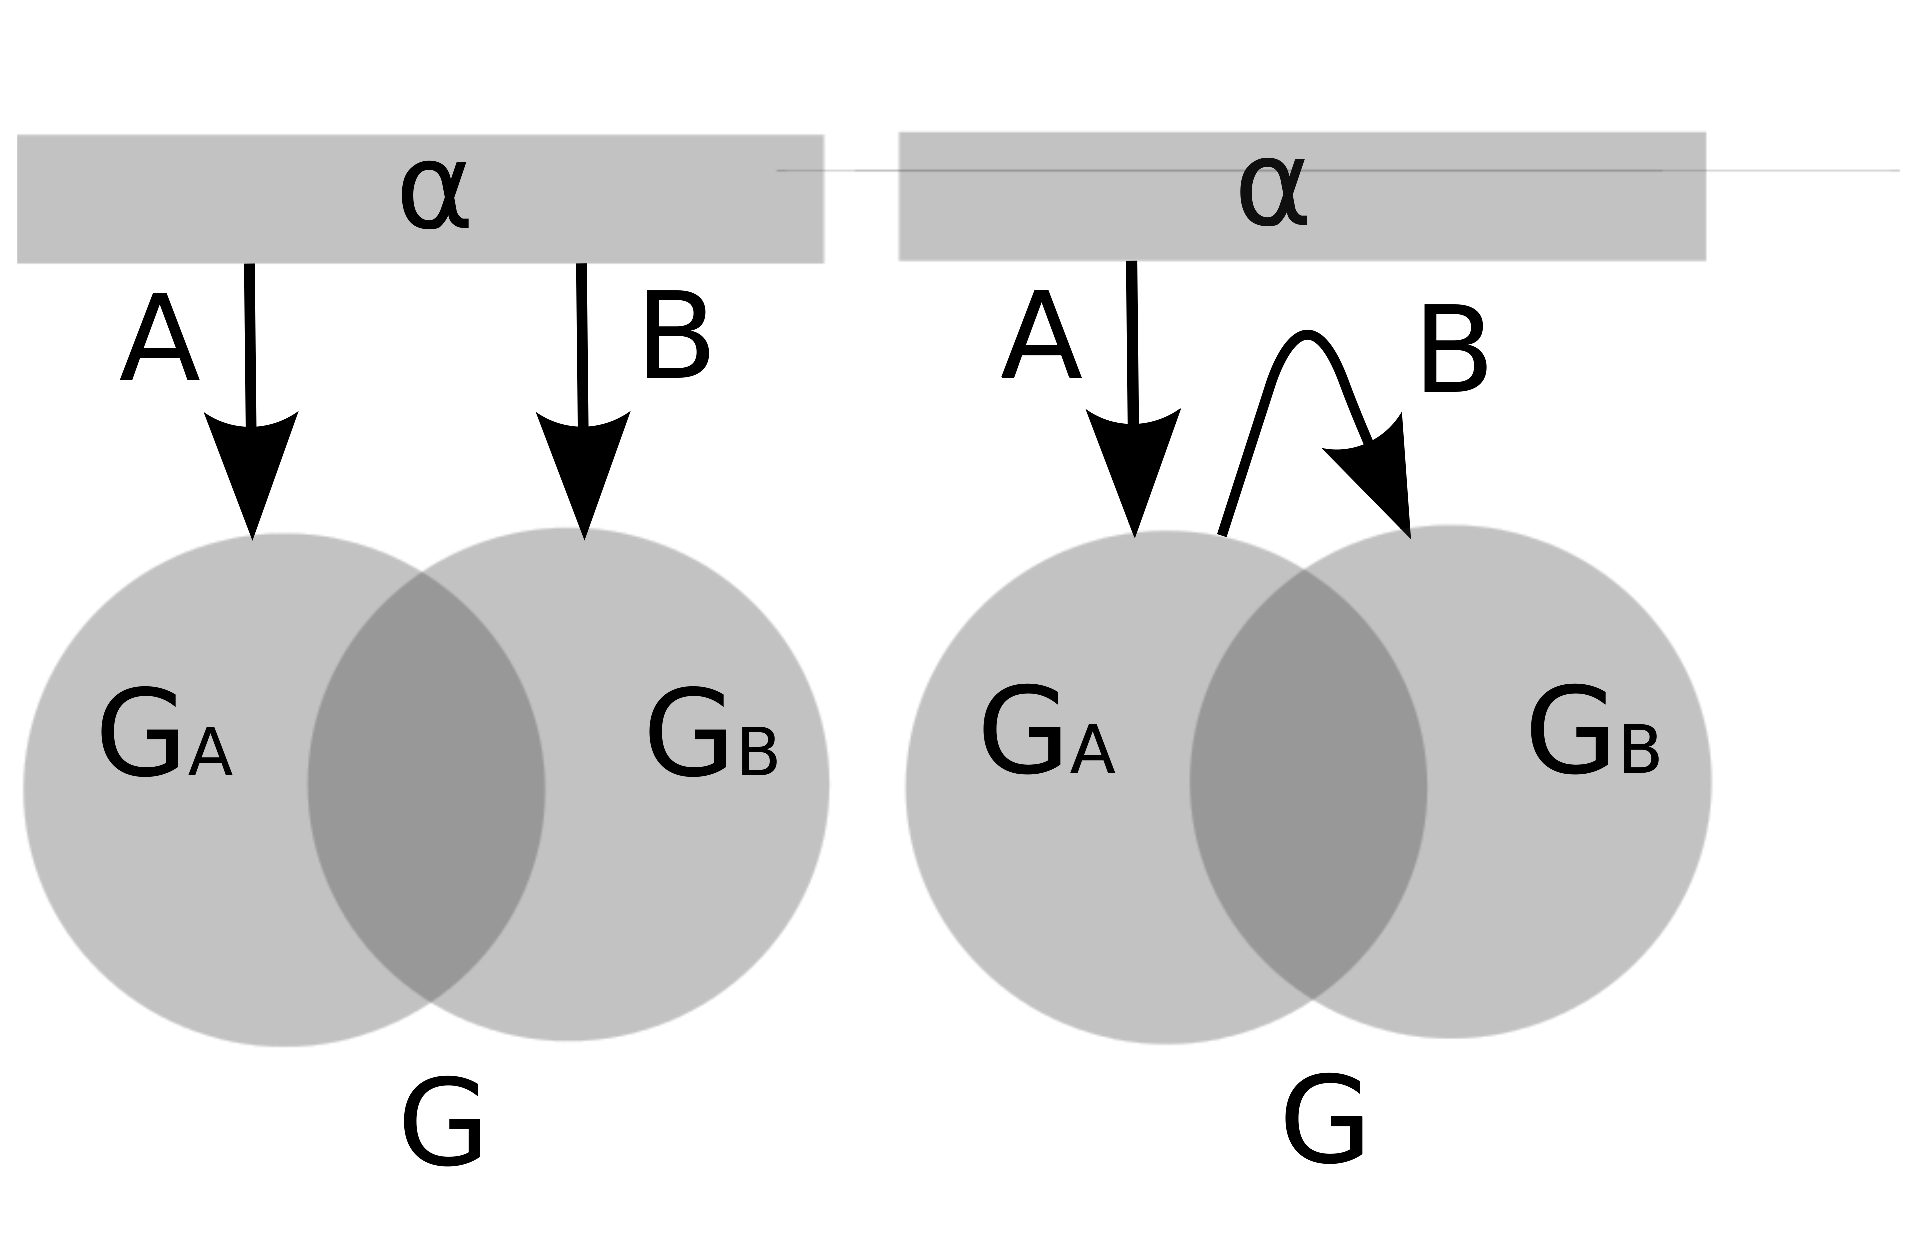
\includegraphics[height=1.18in]{figs/graphmodel2}
  %\label{fig:graph1}}
% %   \hspace{12pt}%
  \caption{Graph model}%
\label{fig:graphmodel2}
\end{minipage}
\begin{minipage}[t]{0.5\linewidth}
%\end{wrapfigure}
%\begin{wrapfigure}{r}{1.0in}
  \centering
% %   %\subfloat[Initially, the owner node $v$ publishes the object]
  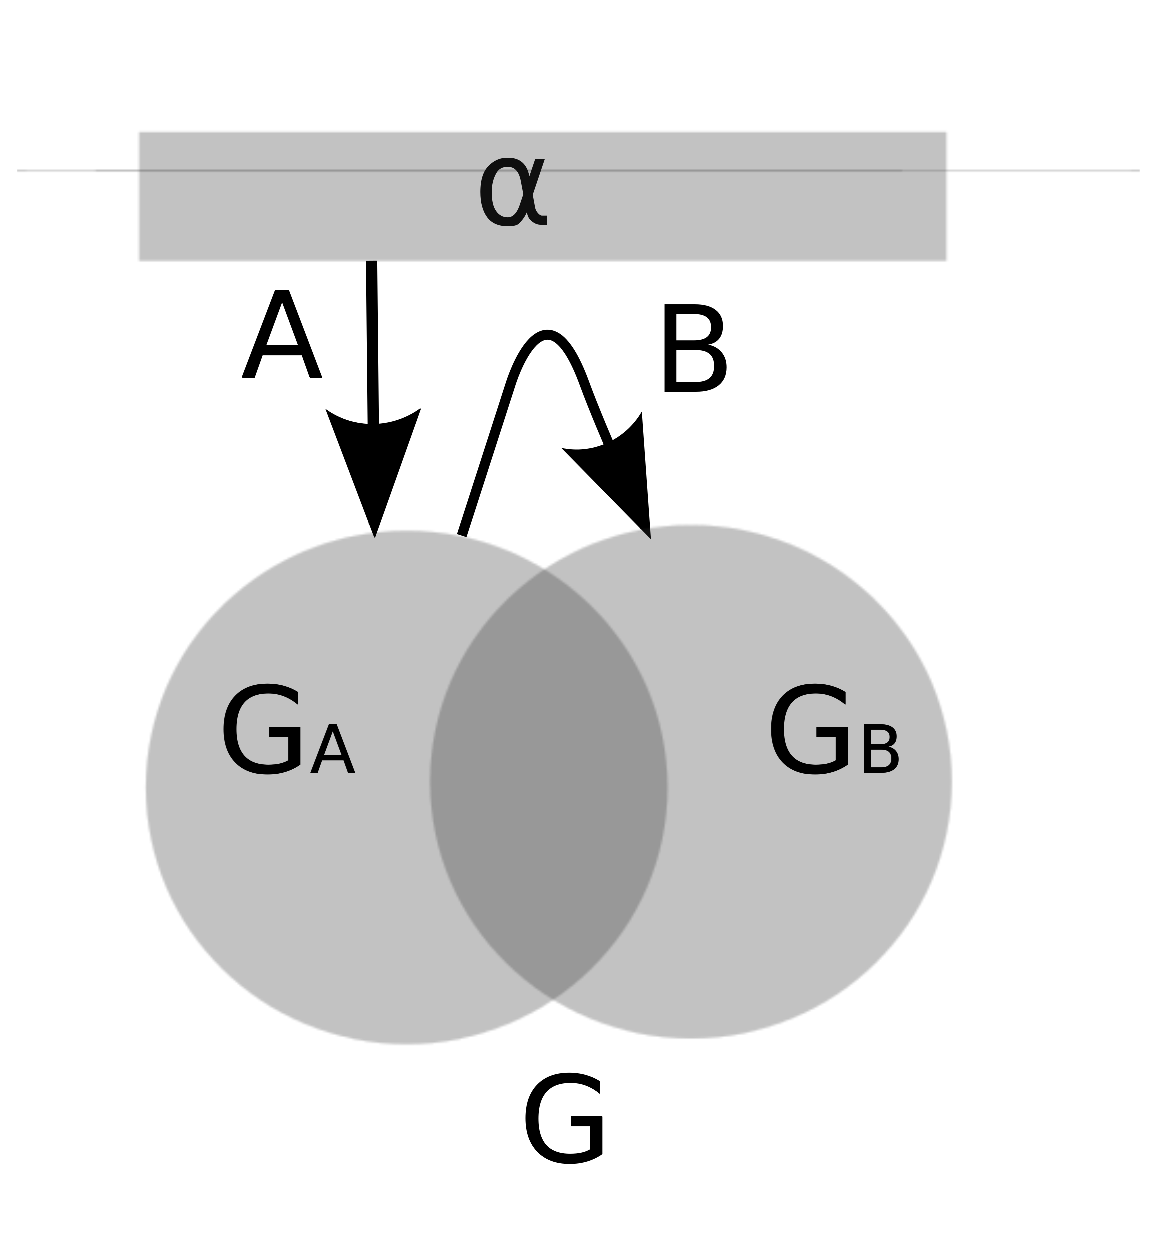
\includegraphics[height=1.18in]{figs/graphmodel2b}
  %\label{fig:graph1}}
% %   \hspace{12pt}%
  \caption{Subgraph model}%
\label{fig:graphmodel3}
\end{minipage}
\end{figure}

Our algorithm uses three phases to perform garbage collection. The three phases are $Phantomize$, $Recover$ and $CleanUp$. The $Phantomization$ phase is a kind of search that marks (i.e. phantomizes) nodes which have lost strong support. The $Recovery$ phase unmarks the nodes, reconnecting the affected subgraph to strong links. If $Recovery$ fails to rebuild links, the $CleanUp$ phase deletes them. The algorithm progresses through all three phases in the order (1. $Phantomize$, 2. $Recover$ and 3. $CleanUp$) and transitions only when there are no more operations left in the current phase. Our algorithm is concurrent because the garbage collection on different subgraphs can proceed independently until, and unless they meet.

If $G$ is the given graph and $\alpha$ is the root set prior to any deletions (see Fig.~\ref{fig:graphmodel2}), $\alpha = \{A, B\}$, and $\alpha = \{ A \}$ after deletions, then
$G$ will become $G_A$, the nodes reachable from $A$.
Thus, $G = G_A \cup G_B$  initially, and
the garbage due to the loss of  $B$ will be $\Gamma_B$.
$$\Gamma_B = G_B - (G_A \cap G_B).$$
During phantomization, all nodes in $\Gamma_B$ and some nodes in $G_A \cap G_B$ will be marked. During recovery, the nodes in $G_A \cap G_B$ will all be unmarked. Hence,
after the $Recovery$ phase, all nodes in $G_A \cap G_B$ will be strongly connected to $A$.
The final phase $CleanUp$ discards the marked memory, $\Gamma_B$.

The above discussion holds equally well if instead of being a root, $B$ is the only strong
link connecting subgraph $G_A$ to subgraph $G_B$. See Fig.~\ref{fig:graphmodel3}.






\begin{theorem}[Cycle Invariant]
\label{theorem:cycleinvariant}
No strong cycles are possible, and all cycles formed in the graph should have at least one weak or phantom edge in the cyclic path.
\end{theorem}
\begin{proof}
This invariant should be maintained through out the graph for any cycles for the algorithm. This property ensures the correctness of the algorithm and the definition of the stable graph. In the rules below, the edge being created is $E$, the source node (if applicable) is called $S$, the target node is $T$. The edge creation rules state: %Assume a graph $G$ that has nodes $a_1$, $a_2$, $a_3$ ... $a_n$. If the edges formed between the nodes create a simple cycle, then by the edge creation rules,
\begin{enumerate}
\setcounter{enumi}{-1}
\item Roots always count as strong edges to nodes.
\item Edge $E$ can be strong if $S$ has no incoming strong edges from other nodes, i.e. if there is no node $C$ with a strong edge to $S$, then $E$ can be created strong. Thus, $S$ is a source of strong edges.
\item A new edge $E$ can be strong if node $T$ has no outgoing non-phantom edges, and $S \neq T$. Thus, $T$ is a terminus of strong edges.
\item A new edge $E$ is strong if $T$ is phantomized and $S$ is not. Thus, $T$ is a terminus of strong edges.
\item A new edge $E$ is weak otherwise. %only if the nodes already have a positive strong count and has outgoing edges, or if it is a self reference.
\item Edge $E$ can only be converted to strong if $T$ is phantomized.
\item A new edge $E$ must be phantom if the node $S$ is phantomized.
\end{enumerate}
Any change described by the above rules regarding strong edges results in one of the nodes becoming a source or terminus of strong edges.
Hence, no strong cycles are possible.
\end{proof}



\begin{theorem}[Termination]
\label{theorem:termination}
Any mutations to a stable graph $G$ will take $\cO(N)$ time steps to form a
new stable graph $G'$, where $N$ is number of edges
in the affected subgraph.
\end{theorem}

\begin{proof}
By {\it stable graph} we mean a graph in which all nodes are strongly connected
from the roots and no phantom links or phantomized nodes are present. Mutations
which enlarge the graph, e.g. adding a root, or edge are constant time
operations since they update the counters and outgoing edge list in a node.
Mutations which diminish the graph, e.g. deleting roots, or edges potentially
begin a process of $Phantomization$, which may spread to any number of nodes in
$G$.


To prove the algorithm is linear we have to prove that each of the three phases in
the algorithm is linear in time. Without loss of generality, consider the graph
in Fig.~\ref{fig:graphmodel2} (or, equivalently, Fig.~\ref{fig:graphmodel3}). In this graph there are two sets of root links
$A$ and $B$ leading into graph $G$. The graph has three components $G_A$, $G_B$,
$G_A \cap G_B$. So,
$$G_A \cap G_B \subset G_A$$ and
$$G_A \cap G_B \subset G_B,$$
where $\pi_A$ and $\pi_B$ are only reachable  by $A$ and $B$, such that
$$\pi_A = G_A - G_A \cap G_B,$$
$$\pi_B = G_B - G_A \cap G_B.$$
$Phantomization$ starts when a node attempts to convert its weak links to
strong, and marks a path along which strong links are lost. $Phantomization$
stops when no additional nodes in the affected subgraph lose strong
support. In Fig.~\ref{fig:graphmodel2} (or Fig.~\ref{fig:graphmodel3}), the marking process will touch at least
$\pi_B$, and at most, all of $G_B$. The marking step affects both nodes and
edges in $G_B$ and ensures that graph is not traversed twice. Thus, $Phantomization$
will take at most $\cO(N)$ steps to complete where
$N$ is the number of edges in $G_B$.

$Recovery$ traverses all nodes in $G_B$ identified during
$Phantomization$. If the node is marked and has a strong count, it unmarks
the node and rebuilds its outgoing edges, making them strong or weak according to
the rules above. The nodes reached by outgoing links are, in turn,
$Recovered$ as well. Since $Recovery$ involves the unmarking of nodes, it is
attempted for every node and edge identified during phantomization, and can
happen only once, and can take at most $\cO(N)$ steps to complete.

Once the $Recovery$ operations are over, then $CleanUp$ traverses the nodes in
the recovery list. For each node that is still marked as phantomized, the node's
outgoing links are deleted. At the end of this process, all remaining nodes will
have zero references and can be deleted. Because this operation is a single
traversal of the remaining list, it too is manifestly linear.
\end{proof}

\begin{theorem}[Safety]
Every node collected by our algorithm is indeed garbage and no nodes reachable by roots are collected.
\label{theorem:safety}
\end{theorem}
\begin{proof}

Garbage is defined as a graph not connected to any roots. If the garbage graph contains
no cycles, then it must have at least one node with all zero reference counts. However,
at the point it reached all zero reference counts, the node would have been collected, leaving
a smaller acyclic garbage graph. Because the smaller garbage graph is also acyclic, it must lose
yet another node. So acyclic graphs will be collected.

If a garbage graph contains cycles, it cannot contain strong cycles by
Theorem~\ref{theorem:cycleinvariant}. Thus, there must be a first node in the
chain of strong links. However, at the point where a node lost its last strong
link, it would have either been collected or phantomized, and so it can not
endure. Since there no first link in the chain of strong links can endure, no
chain of strong links can endure in a garbage graph. Likewise, any node having only weak incoming
links will phantomize. Thus, all nodes in a garbage graph containing cycles
must eventually be phantomized.

If such a state is realized, $Recovery$ will occur and fail, and $Cleanup$
will delete the garbage graph.

Alternatively, we show that an object reachable from the roots will not be collected.
Suppose $V^C$ is a node and there is an acyclic chain of nodes
$ Root \rightarrow ... \rightarrow V^A \rightarrow V^B \rightarrow ... \rightarrow V^C$.
Let $V^A$ be a node that is reachable from a root, either directly or by some chain of references.
If one of the nodes in the chain, $V^B$, is connected to $V^A$
and supported only by weak references, then
at the moment $V^B$ lost its last strong link it would have phantomized and converted any
incoming weak link from $V^B$ to strong. If $V^B$ was connected by a phantom link from $V^A$,
then $V^B$ is on the recovery list and will be rebuilt in $Recovery$. This logic can be
repeated for nodes from $V^B$ onwards, and so $V^C$ will eventually be reconnected by
strong links, and will not be deleted.
\label{safety}
\end{proof}

\begin{theorem}[Liveness]
\label{theorem:liveness}
For a graph of finite size, our algorithm eventually collects all unreachable nodes.
\end{theorem}
\begin{proof}
We say that a garbage collection algorithm is $live$ if it eventually collects
$all$ unreachable objects, i.e. all unreachable objects are collected and never
left in the memory.


The only stable state for the graph in our garbage collection is one in which all nodes
are connected by strong links, because any time the last strong link is lost a chain of
events is initiated which either recovers the links or deletes the garbage. Deletion of
a last strong link can result in immediate collection or $Phantomization.$ Once $Phantomization$
begins, it will proceed to completion and be followed $Recovery$ and $Cleanup.$ These
operations will either delete garbage, or rebuild the strong links. See Theorem~\ref{theorem:safety}.
%\end{comment}
\end{proof}

Note that the live system may create objects faster than the
$Phantomization$ phase can process. In this case, the $Phantomization$ phase will
not terminate.
However, in Theorem \ref{theorem:liveness} when we say the graph be ``of finite size'' we
also count nodes that are unreachable but as yet uncollected,
which enables us to bound the number of nodes that are being added while the $Phantomization$ is in progress.
%, and it is for this
%objection, and similar objections, that we added the qualification that the
%graph be of finite size.
On a practical level, it is possible for garbage to be
created too rapidly to process and the application could terminate with an out-of-memory error.


\subsection{Experimental Results}
\label{section:experimental}
To verify our work, we modeled the graph problem described by our garbage
collector in Java using fine-grained locks. Our implementation simulates the mutator and collector
behavior that would occur in a production environment. Our mutator threads create, modify, and
delete edges and nodes, and the collector threads react as necessary. This prototype
shows how a real system should behave, and how it scales up with threads.

We also developed various test cases to verify the correctness of the garbage
collector implementation. Our test cases involve a large cycle in which the root
node is constantly moved to the next node in the chain (a ``spinning wheel''), a doubly linked list
with a root node that is constantly shifting, a clique structure, and various
tests involving a sequence of hexagonal cycles connected in a chain.

In Fig.~\ref{fig:scale} we
collected a large number of hexagonal rings in parallel. This
operation should complete in time inversely proportional to the number of threads
in use, as each ring is collected
independently. The expected behavior is observed.

In Fig.~\ref{fig:overhead} we performed the same test, but to a set
of connected rings. The collection threads
merge, but not immediately, so the collection time goes down with the number of
threads used, but not proportionally because the
collection threads only operate in parallel part of the time.

In Fig.~\ref{fig:linearity}, we perform tests to see whether our garbage
collector is linear. We considered a clique, two different hexagonal cycles (one
is interlinked and other separate), a doubly-linked list, and simple cycles, and
measured the collection time per object by varying the size of the graph and
fixing the collector threads to two all times. The results confirmed that our
collector in indeed linear in time.

Our tests are performed on two 2.6 GHz 8-Core Sandy Bridge Xeon Processors (i.e.
on 16 cores) running Redhat Linux 6 64-bit operating system.

\begin{figure}[h!]
  \centering
% %   %\subfloat[Initially, the owner node $v$ publishes the object]
  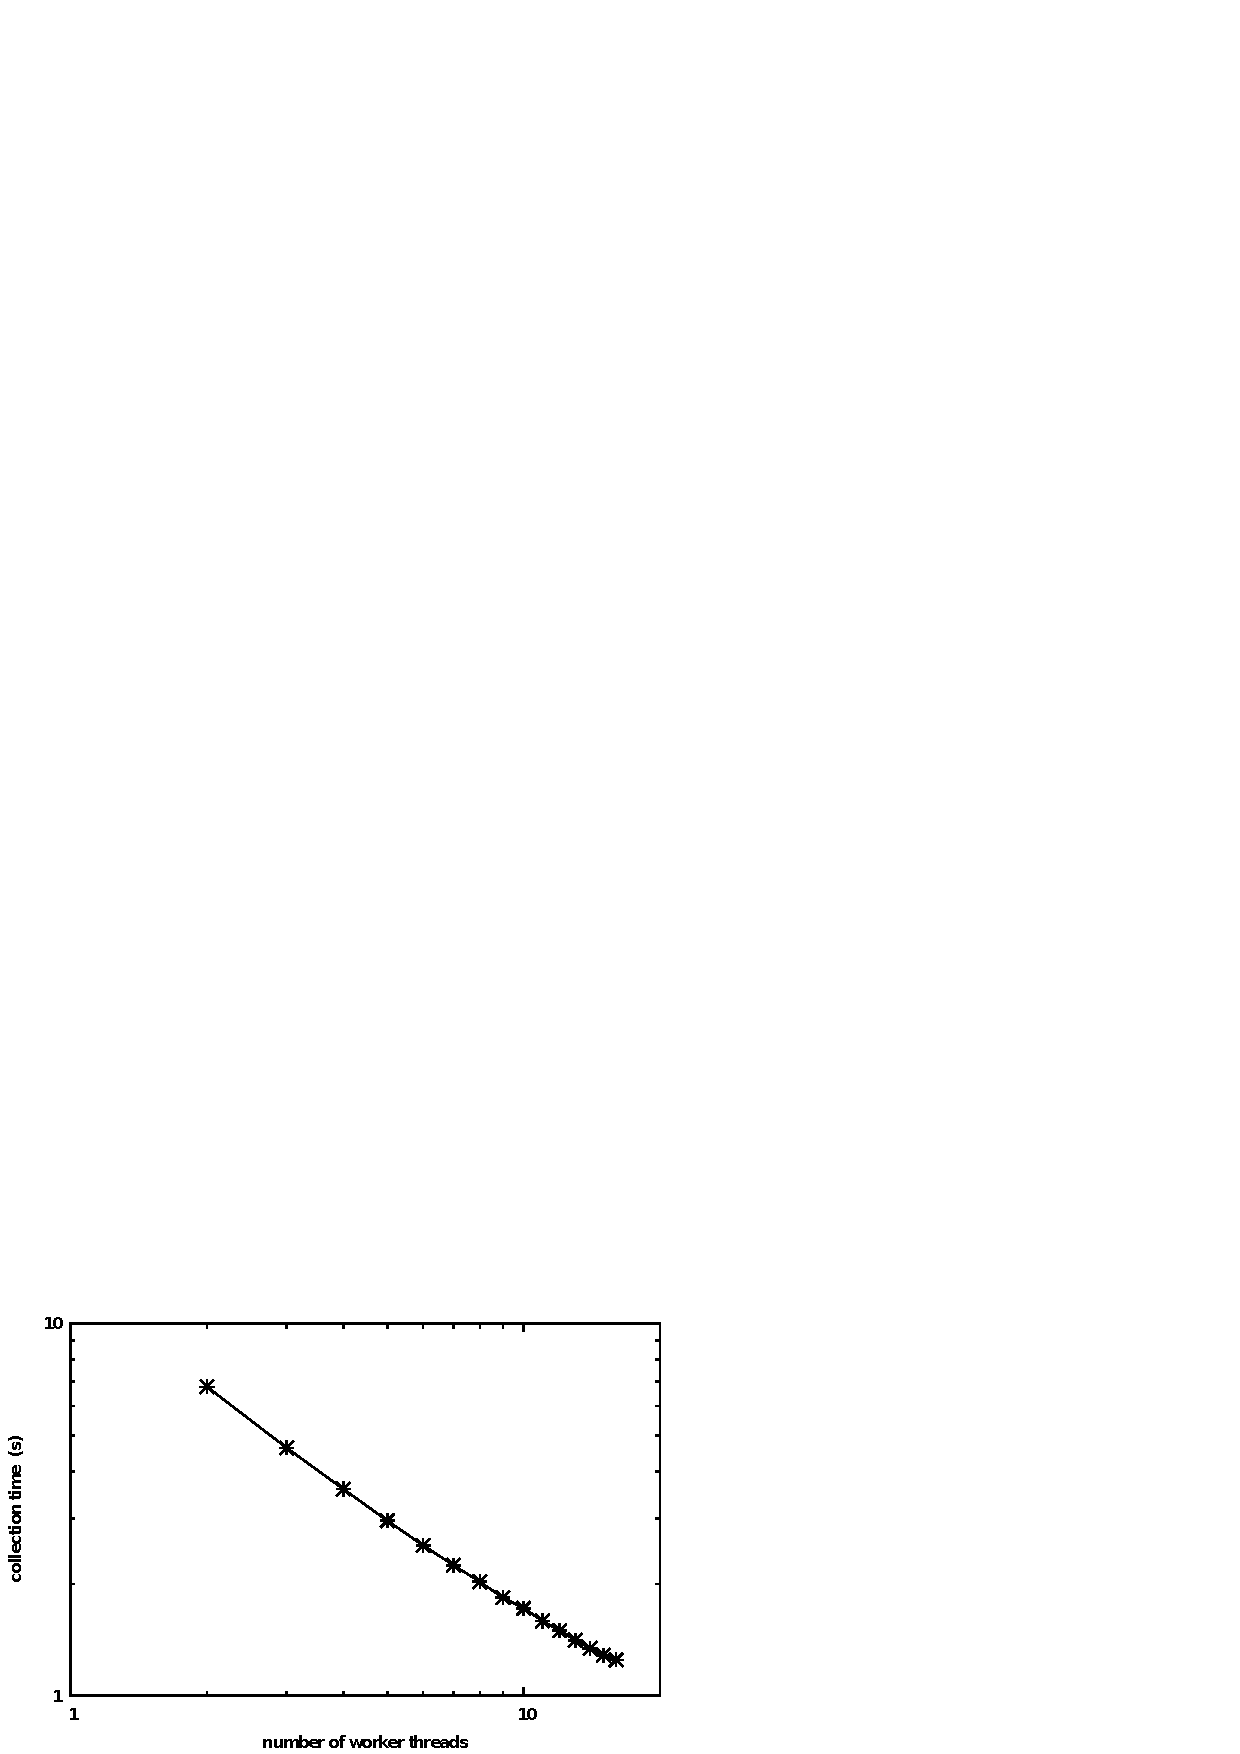
\includegraphics[height=1.8in,width=3.0in]{figs/CleanupTimeperObjectonly16log}
  %\label{fig:graph1}}
% %   \hspace{12pt}%
  \caption{
  A large number of independent rings are collected by various number of
  worker threads. Collection speed drops linearly with the number of
  cores used.
  }
   \label{fig:scale}
  \end{figure}

% % While the algorithm can scale very well with the independent sets, the collector threads working on the shared structure needs synchronization. The testcase that we used for scaling is changed so that all benzene structures are interlinked and collector has to communicate and coordinate their activities based on other collector threads. The algorithm systematically achieves optimized communication and coordination among the multiple collector threads working on the same shared structure. As a result of this, the Fig \ref{fig:overhead} shows the synchronization issues due to multiple threads interacting among each other to cleanup the structure.
\begin{figure}[h!]
  \centering
% %   %\subfloat[Initially, the owner node $v$ publishes the object]
  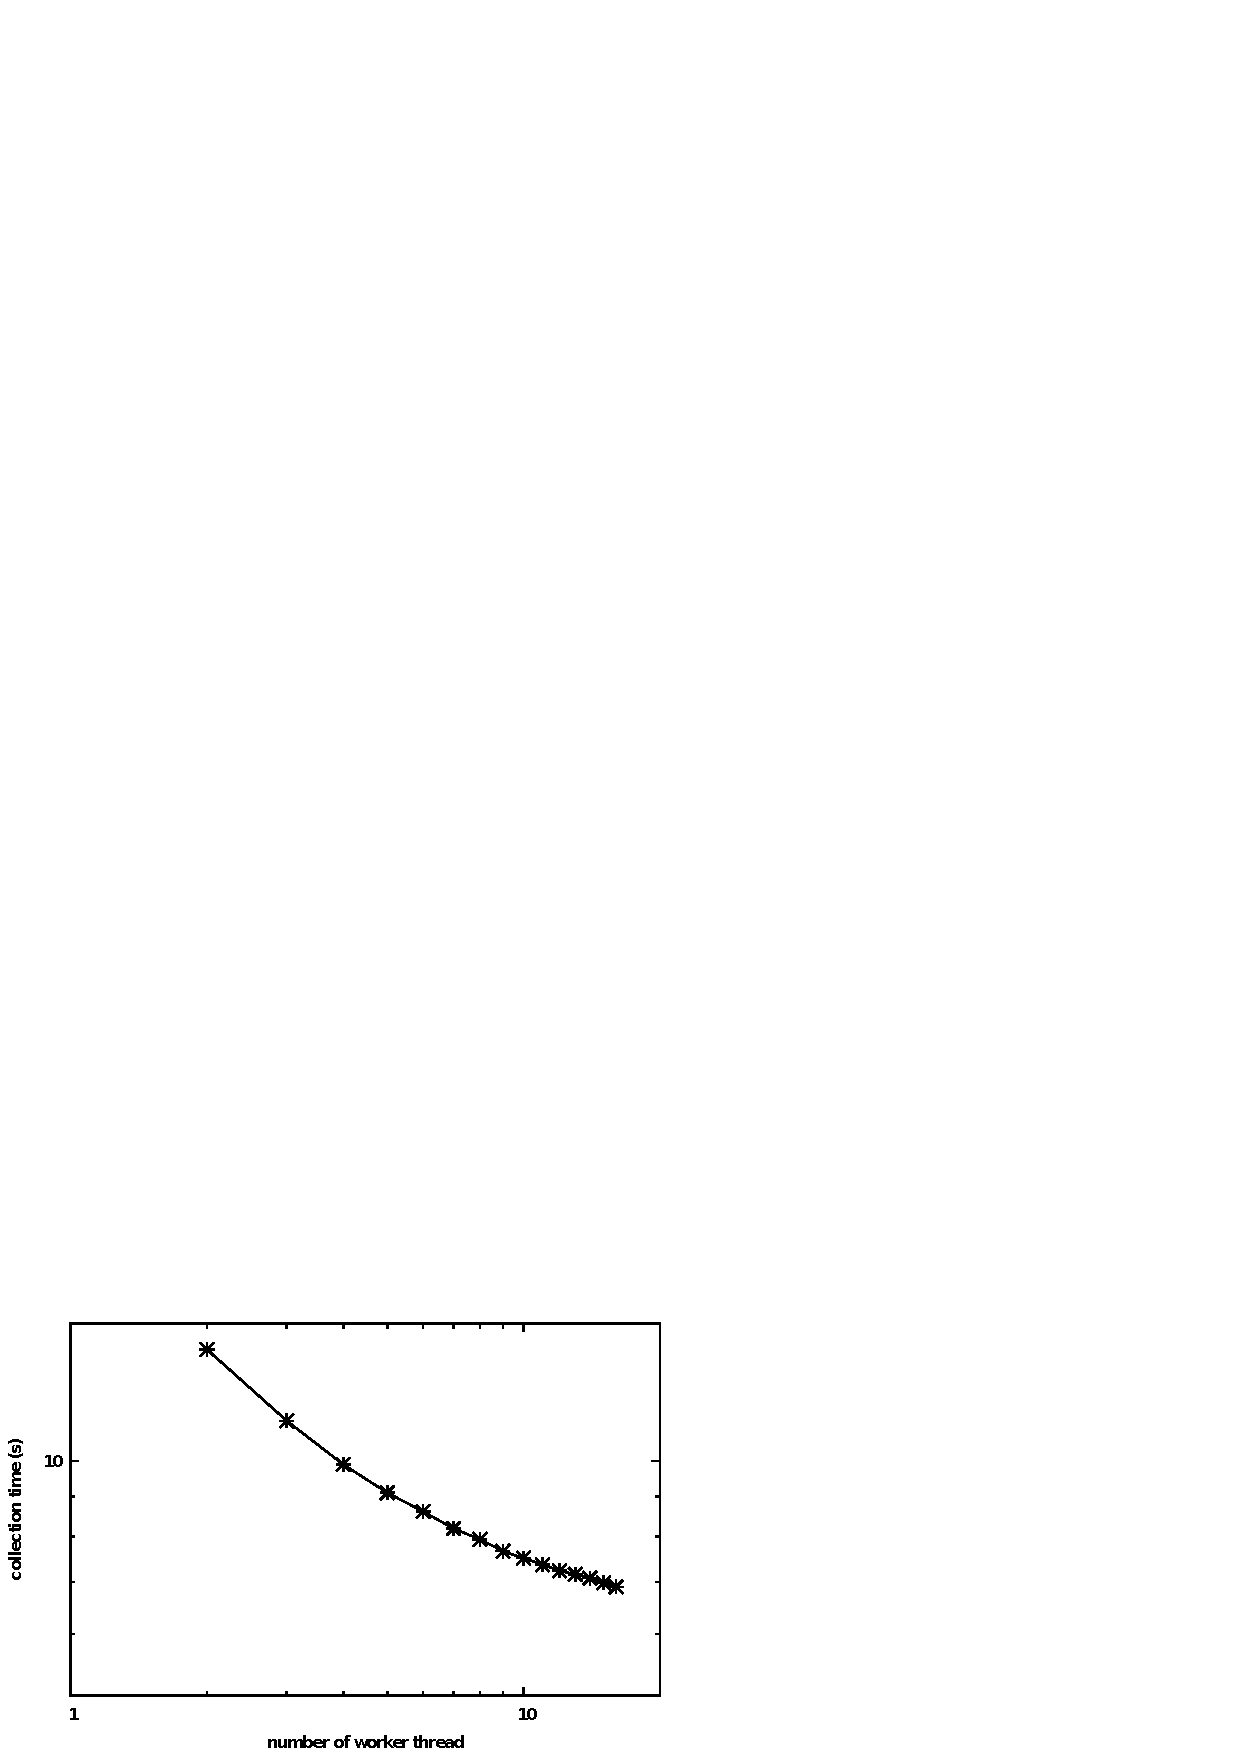
\includegraphics[height=1.8in,width=3.0in]{figs/collapseoverheadonly16log}
  %\label{fig:graph1}}
% %   \hspace{12pt}%
  \caption{A chain of linked cycles is created in memory. The connections are severed,
  then the roots are removed. Multiple collector threads are created and operations
  partially overlap.}
   \label{fig:overhead}
  \end{figure}


\begin{figure}[h!]
  \centering
% %   %\subfloat[Initially, the owner node $v$ publishes the object]
  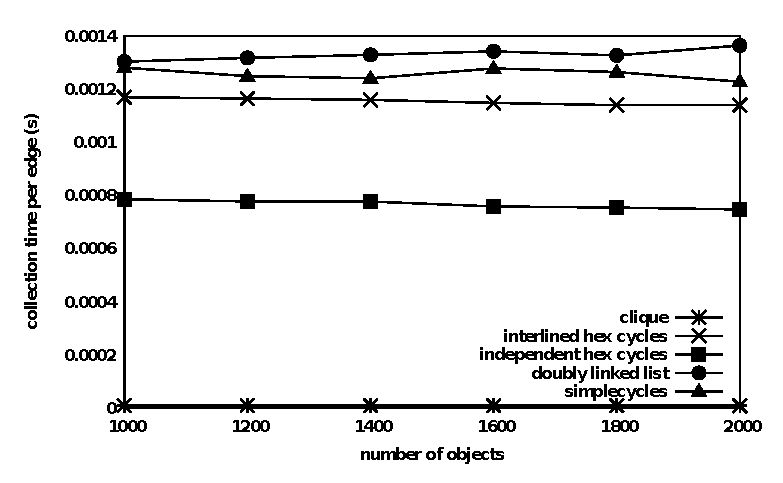
\includegraphics[height=1.8in,width=3.0in]{figs/linearity}
  %\label{fig:graph1}}
% %   \hspace{12pt}%
  \caption{
  Graphs of different types are created at various sizes in memory,
  including cliques, chains of cycles, large cycles, and large doubly
  linked lists. Regardless of the type of object, collection time
  per object remains constant, verifying the linearity of the underlying
  collection mechanism.
  }
   \label{fig:linearity}
  \end{figure}
